\documentclass{book}
\usepackage[margin=1in,footskip=0.25in]{geometry}
\usepackage[toc,page]{appendix}

% for glossaries
\usepackage[xindy]{glossaries}

% for figures
\usepackage{graphicx}

% this command generates the glossary:
\makeglossaries
\loadglsentries{acronyms.tex}

% Improved C++ logo
\newcommand{\CC}{C\nolinebreak\hspace{-.05em}\raisebox{.4ex}{\tiny\bf +}\nolinebreak\hspace{-.10em}\raisebox{.4ex}{\tiny\bf +}}

% Footer with author names of the work
\usepackage{fancyhdr}
\pagestyle{fancy}
\fancyhead{} % clear all header fields
\renewcommand{\headrulewidth}{0pt} % no line in header area
\fancyfoot{} % clear all footer fields
\fancyfoot[LE,RO]{\thepage}           % page number in "outer" position of footer line
\fancyfoot[RE,LO]{Dematties D, Rizzi S, Thiruvathukal, GK, Wainselboim, AJ. and Zanutto, BS}

\begin{document}
%\tableofcontents

%\chapter{Regular Chapter}
\begin{appendices}

\chapter{Computational Setup}
\label{Comp_setup}

In this appendix we include the Computational Setup of our \gls{cstm}, which describes its object-oriented design as well as the parallelization strategy used for its implementation in \gls{hpc} resources. This appendix also includes preliminary Strong and Weak Scaling tests of our code on \gls{hpc} resources.


\section{Inheritance and Compositional Structure}

We implemented our algorithms in standard \CC14 using the \gls{oop} paradigm in a set of classes interrelated by inheritance and composition. We implemented proximal afferent and distal inter-columnar connectivity as well as minimum-maximum margins in afferent synaptic weights in the \glsfirst{el} class. We configured such class as a composition of objects of class \glsfirst{csom}. The main member in the \gls{el} class is a \gls{stl} vector of \gls{csom} objects. A complete diagram of the hierarchical inheritance and compositional structure of the implementation can be seen in Fig. \ref{fig:Skeleton}.

\begin{figure}[h!]
    \centering
    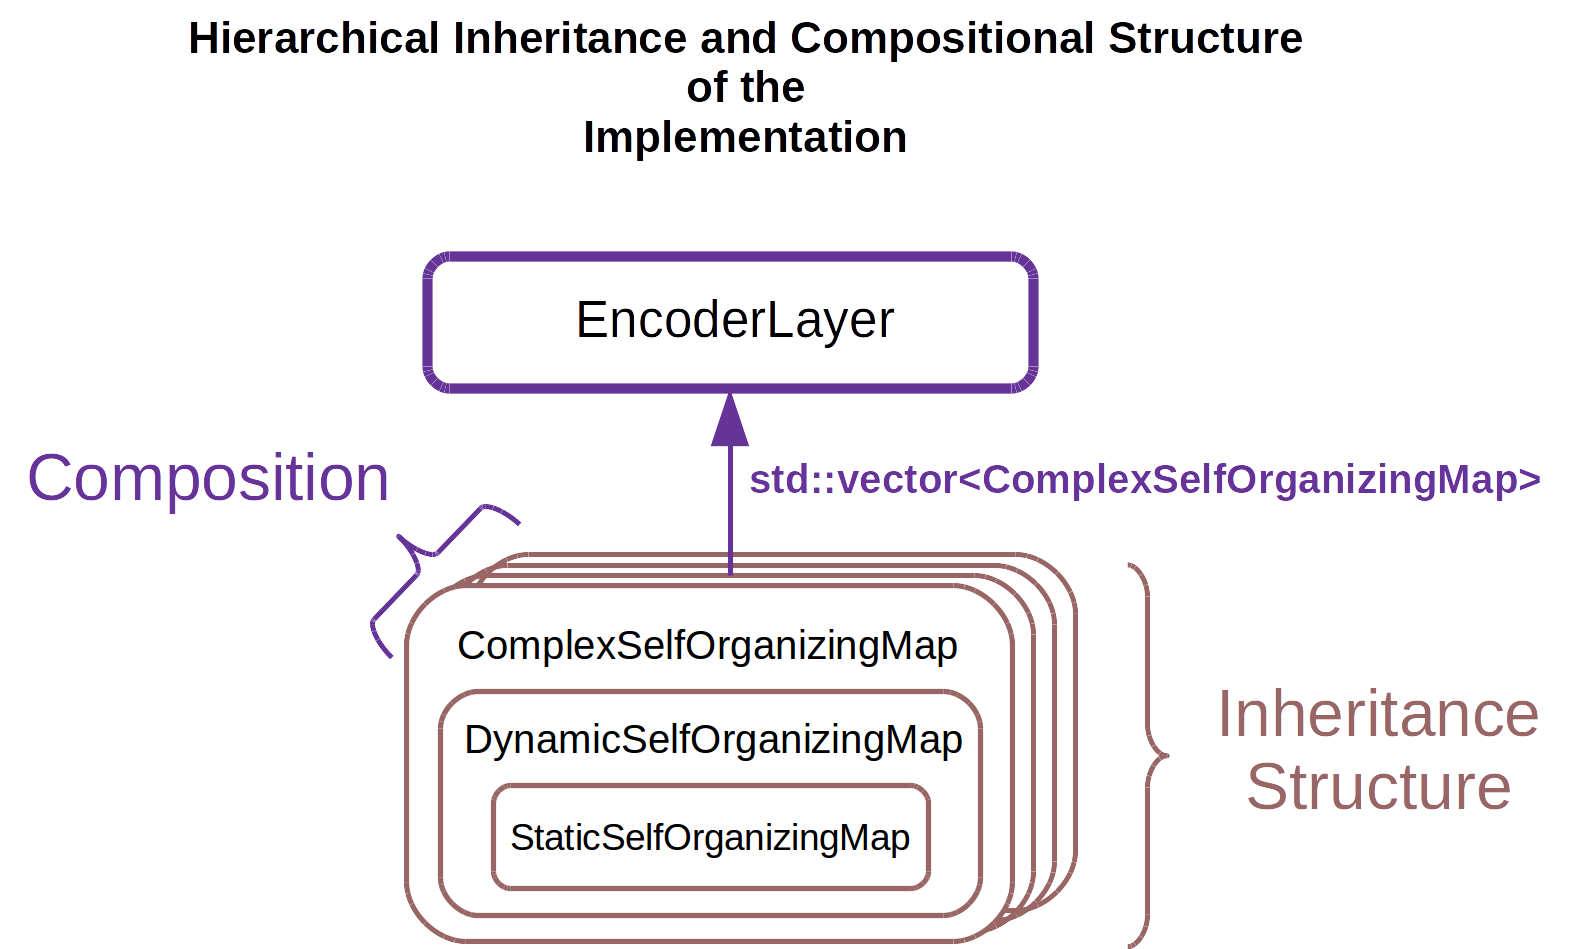
\includegraphics[width=0.8\textwidth]{Skeleton.png}
    \caption{Hierarchical Inheritance and Compositional Structure of the Model Implementation.
    \glsfirst{csom} inherits from \glsfirst{dsom} which inherits from \glsfirst{ssom}.
    The \glsfirst{el} is formed by the composition of a set of \glspl{csom} gathered
    in a std::vector \glsfirst{stl} container.}
    \label{fig:Skeleton}
\end{figure}

\section{\glsfirst{el} Parallelization}

We parallelized the \gls{el} class by means of a hybrid \gls{mpi}+\gls{omp} paradigm. We distributed \glspl{csom} among \gls{mpi} ranks as a deck of cards is distributed among different players. Each \gls{mpi} rank ends up with one or more \glspl{csom} and the \glspl{csom} in each rank are distributed among different \gls{omp} threads (Fig. \ref{fig:EncoderParallelization} A and B respectively). Information among \gls{mpi} ranks must be transferred in each time step. We gather all the information corresponding to the \glspl{csom} in each rank and then use \gls{mpi} Bcast function to transmit such information using a special comunication protocol by means of which we specify the boundaries in the information corresponding to each \gls{csom}(Fig. \ref{fig:EncoderParallelization} C). By means of this strategy each \gls{mpi} rank has to call \gls{mpi} Bcast just once in order to transmit its data. The \gls{el} uses \gls{mpi} I/O parallel file system to save its status in Matlab/Octave format (Fig. \ref{fig:EncoderParallelization} D). Each \gls{mpi} rank gathers all the data corresponding to its \glspl{csom} in the \gls{el} and communicates the part of the file it will use to the other \gls{mpi} ranks, in order to store the data without interfering with the other ranks in the \gls{mpi} environment. Then, each \gls{mpi} rank saves all its data with a unique call to \gls{mpi} Write. 

\begin{figure}[h!]
    \centering
    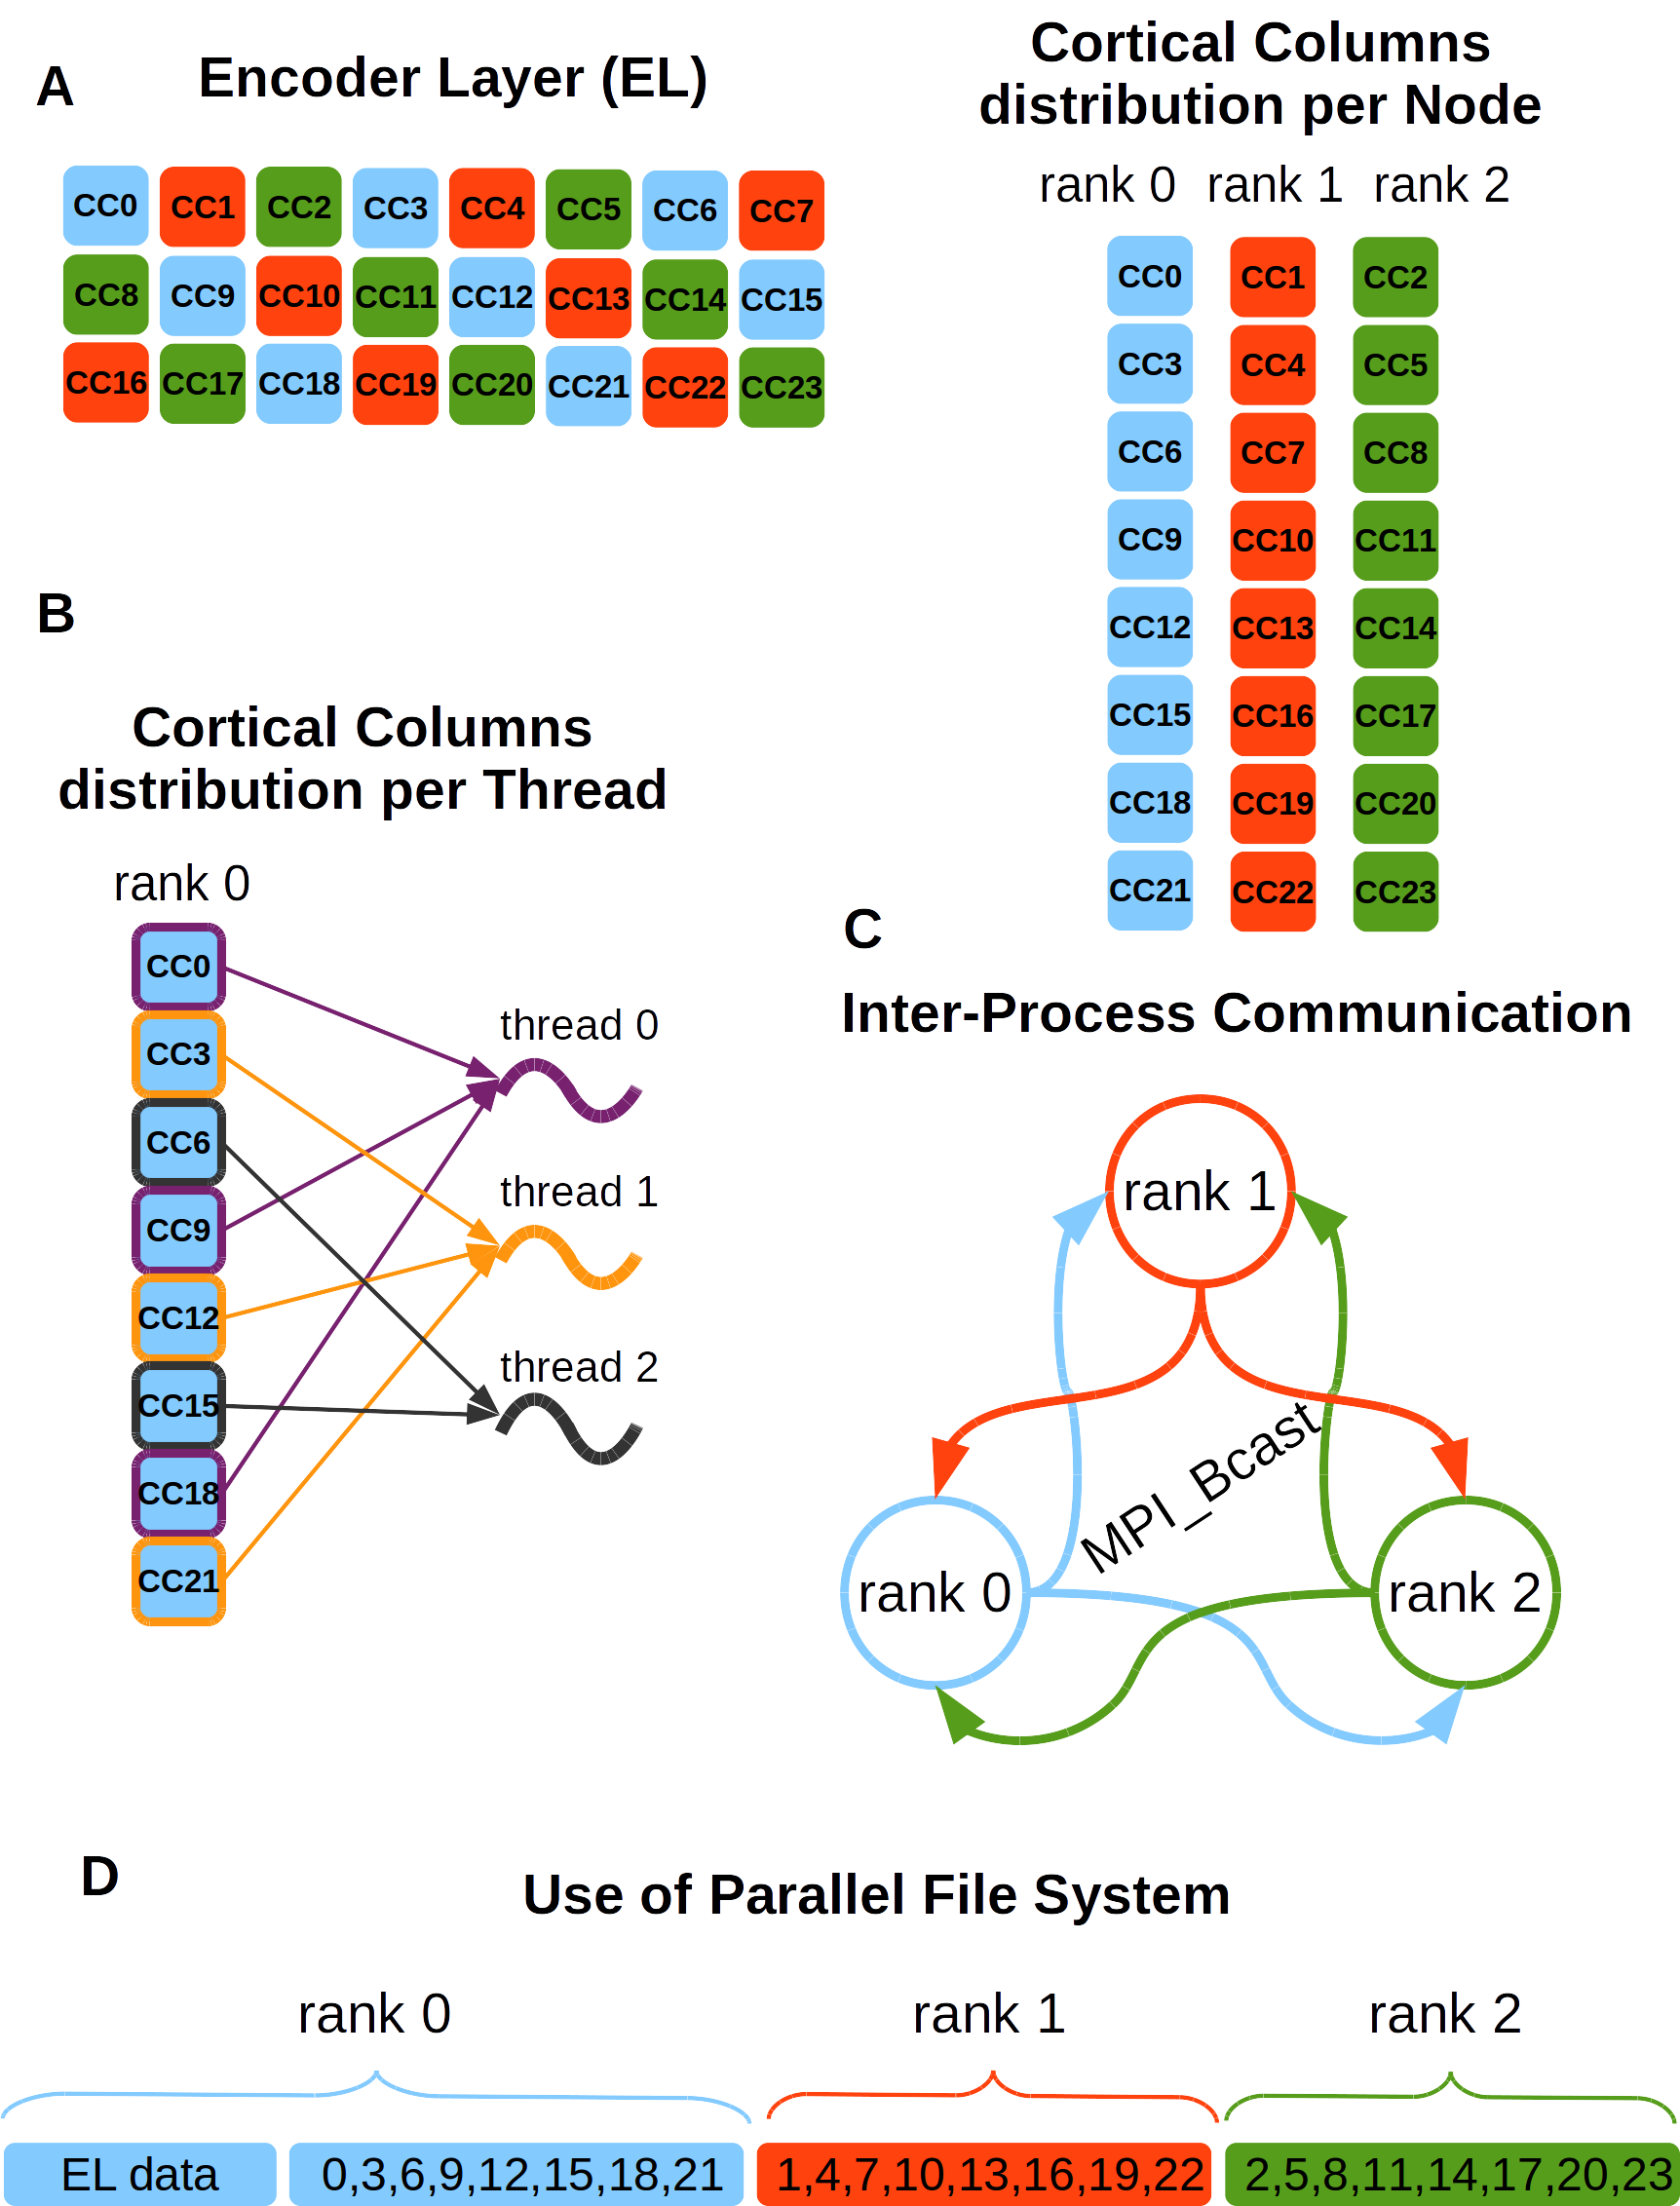
\includegraphics[width=0.75\textwidth]{EncoderParallelization.png}
    \caption{\glsfirst{el} \gls{mpi}+\gls{omp} parallelization. (A) Distribution of \gls{csom} objects in an \gls{el} with
    3 by 8 (24) \glspl{cc} among three \gls{mpi} ranks with three \gls{omp} threads per rank.
    Certain ranks could take care of a different number of
    \glspl{csom} depending on the number of \gls{mpi} ranks as well as the number of \glspl{cc} in the \gls{el}.
    (B) Each \gls{mpi} rank distributes its \glspl{csom} among different threads in the same fashion.
    (C) \gls{mpi} \gls{ipc} among different ranks. \gls{ipc} is carried out at each time step since each \gls{mpi} rank 
    requires the complete \gls{el} output at each time step.
    Each \gls{mpi} rank broadcasts the information corresponding to its \glspl{cc} to the other ranks in the \gls{mpi}
    environment.
    (D) \gls{el} information distribution in a file to save its status.
    Each \gls{mpi} rank puts the formated data corresponding to its \glspl{csom} in a \gls{stl} stringstream class template.
    Rank 0 also takes care of the \gls{el} structure, connectivity and parameters.
    Once each rank has its stringstream with the formated data, it communicates its file view to the other ranks.
    Then each rank writes its stream of bytes in parallel without interfering with other ranks in the \gls{mpi} environment.
    An \gls{el} with a different number of ranks can load the same file without affecting the final results.
    Each rank in the new \gls{el} loads the complete file in a \gls{stl} stringstream class template and then takes the
    informations that concern it from such structure.}
    \label{fig:EncoderParallelization}
\end{figure}

The implementation has Checkpoint and Restart capacity in its training stage where there is total flexibility in terms of the number of ranks with which the execution is restarted. A cortical layer could have been saved with $n$ ranks and such layer could be restarted with $m$ ranks without affecting the final results.

It is important to note that the number of \glspl{cc} shown in Fig. \ref{fig:EncoderParallelization} is merely illustrative and does not reflect the real numbers in terms of computational resources used for this implementation. 

We performed all computational experiments on Cooley, a visualization and analysis cluster at Argonne National Laboratory. We ran the simulations using 25 nodes (9 \glspl{cc} per node and one node per \gls{mpi} rank) and 9 OpenMP threads per node/rank (one thread per \gls{cc}).

\section{Initial Strong and Weak Scaling Tests on Cooley}

Beyond the notion that our computational approach is intended to be applied in leadership supercomputers in the future, in the present work an essential step is to test our code in order to see how it uses the resources provided by Cooley Nodes. Parallel scalability is a measurement that indicates how efficient is our code when using increasing numbers of parallel processing elements--Nodes or Processes and \glspl{cpu} or Threads on Cooley. Fig. \ref{fig:Strong_Weak} shows the scaling capacity of our code in terms of run time vs. number of processing elements used for the task. In our tests we always constrain our code to run one \gls{mpi} rank per Cooley node. Each \gls{mpi} rank spreads an specific number of threads through the different \glspl{cpu} in its corresponding node (Fig. \ref{fig:EncoderParallelization} A and B). There are two ways to measure the parallel performance of a given application. The measure to be applied will depend on whether the application is \gls{cpu}-bound or memory-bound. Such measurements are referred to as \emph{strong} and \emph{weak} scaling, respectively.

\begin{figure}[h!]
    \centering
    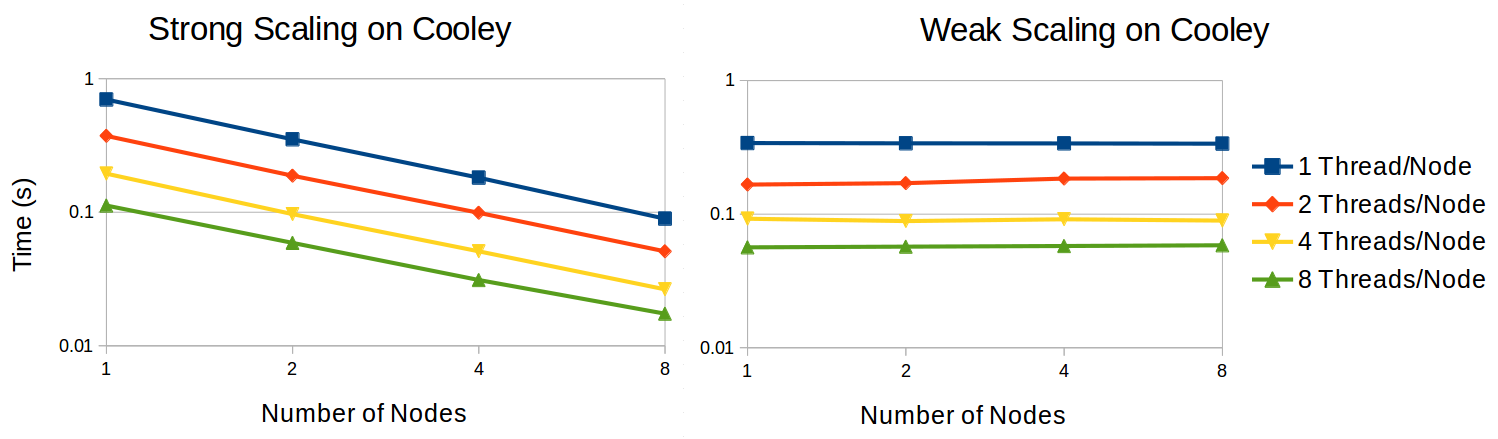
\includegraphics[width=1.0\textwidth]{Strong_Weak.png}
    \caption{Strong and Weak scaling tests on Cooley nodes. Left: Strong scaling. Run time vs. the number of nodes for different number of threads per node.
	    The problem size stays fixed but the number of processing elements are increased.
    Right: Weak scaling. Run time vs. the number of nodes for different number of threads per node.
    In this case the problem workload assigned to each processing element stays constant and additional elements are used to solve a larger total problem (i.e. a problem that would not fit in the available RAM on a single node).}
    \label{fig:Strong_Weak}
\end{figure}

Straight lines in Fig. \ref{fig:Strong_Weak} (left) show an initially good strong scalability of our code while the small slope exhibited by Fig. \ref{fig:Strong_Weak} (right) allows us to foresee a good weak scaling performance of our code in high end leadership supercomputers.

\chapter{Encoder Layer parameters swept}
\label{EL_Parameters_Swept}

This appendix includes a battery of complementary experiments showing the classification accuracy levels of different instances of the \gls{el} in the \gls{cstm}.

\section{Word Classification Performance Tests}

The \gls{el} has shown exceptional classification performance. In order to attain the appropriate configuration on the parameters describing the structure of the model, we produced a swept of models with different sizes in the \gls{el}. We progressively increased the number of cortical columns (CCs) as well as the distal receptive fields in the \gls{el} and tested the corresponding phonetic classification performances.

In Fig.~\ref{fig:WordClassification2} we show the initialization parameters for the different \glspl{el}.

\begin{figure}[h!]
    \centering
    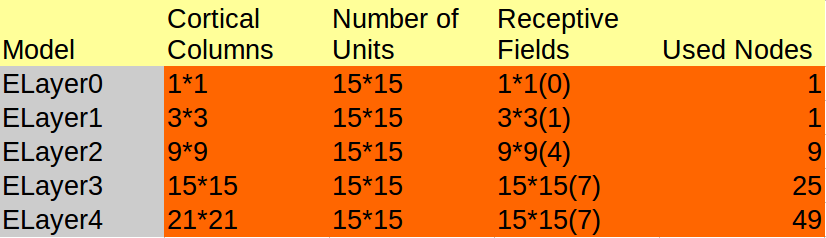
\includegraphics[width=1.0\textwidth]{WordClassification2.png}
    \caption{\gls{el} parameters swept. The number of \glspl{cc} goes from 1 to 441 in 4 steps. The receptive fields go from 1 to 225 \glspl{cc} in 4 steps too. The number of neural units in each \gls{cc} is kept constant and the number of compute nodes to run the models is varied appropriately in order to get a fair distribution of \glspl{cc} in each compute node.}
    \label{fig:WordClassification2}
\end{figure}


The \gls{el}0 had one CC with 15 for 15 (225) Neural Units, the \gls{el}1 had an array of 3 for 3 (9) CCs with 225 Neural Units and so on. As depicted by the figure, a receptive field of 1 for 1 corresponds to a parameter of 0 and represents a receptive field of one CC. This means that each CC has lateral distal connections only with itself. A receptive field of 3 for 3 represents the fact that each CC can be distally connected with 9 CCs around it, including itself. For each \gls{el} we used a number of nodes as to try to run 9 CCs per Node distributed by means of OpenMP multi-threading operations.

Fig.~\ref{fig:WordClassification3} shows the average phonetic word classification performance obtained by each \gls{el}. As can be seen in the figure, even the smallest instance of the \gls{el} (the \gls{el}0) outperformed the \gls{mrstsa} algorithm in the word classification task. This supports our hypothesis that the improvement in the performance comes from the algorithmic sequential characteristics of the \glspl{el}.

\begin{figure}[h!]
    \centering
    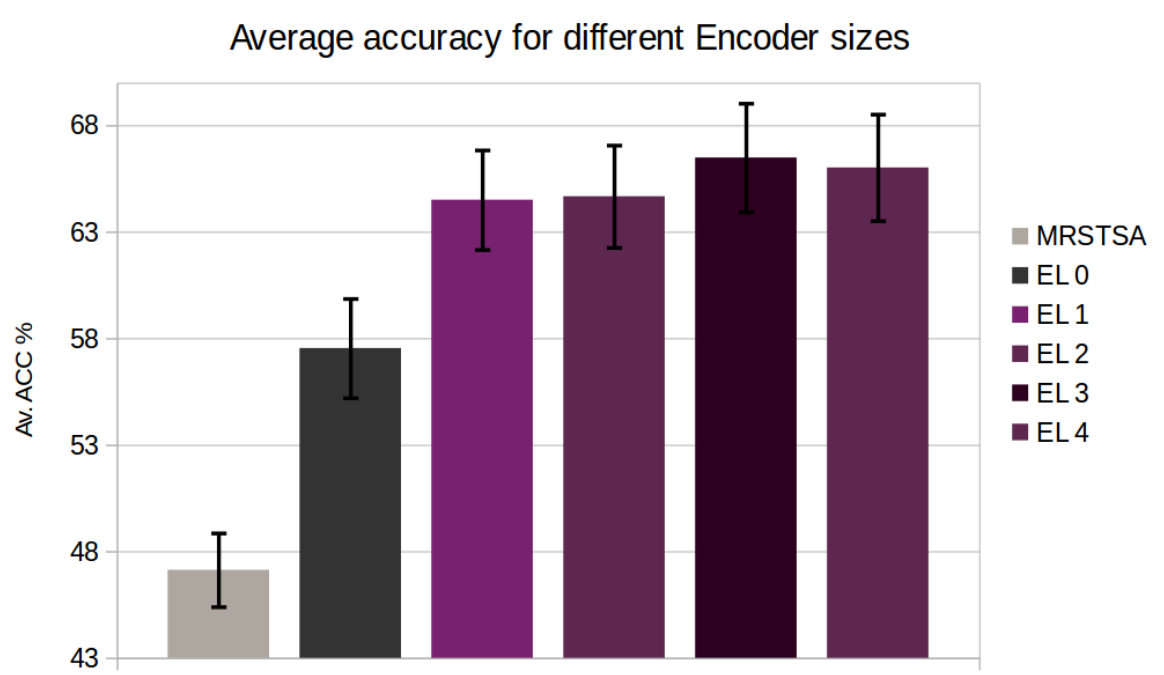
\includegraphics[width=1.0\textwidth]{WordClassification3.png}
    \caption{Classification Accuracy for the \gls{mrstsa} and for different instances of the \gls{el}.}
    \label{fig:WordClassification3}
\end{figure}

From Fig.~\ref{fig:WordClassification3}, a clear tendency of the performance can also be seen where the classification accuracy grows with the size of the 4 first \glspl{el}. Bigger models with larger numbers of \glspl{cc} present more phonetic hypotheses which could allow better probabilistic inference in the sequential processing task. It is also known that smaller models suffer from a distal dendrite sparsity which generates repetitive \glspl{mfe} and a lack of \glspl{sdr} whose origins are prediction faults produced in the processing of the stream of data. In this way, a modification in some parameters of the model, could affect others in unpredictable ways and a comprehensive study of such phenomena far exceeds the purpose of the current research. Regardless of that, we consider that the present battery of experiments shows a sound initial parameter configuration as to pose an appropriate \gls{el} arrangement.

\section{Experimental Data to Run the Tests}

For the entire collection of experiments we generated corpora of 500 words with mono, di and trisyllabic English words with vocabularies of five words using Festival Text to Speech Synthesis.

The vocabularies used including the following:

\begin{itemize}
	\item Monosyllabic vocabulary: \textit{map, dog, mouse, with} and \textit{truck}.
	\item Disyllabic vocabulary: \textit{answer, doctor, teacher, summer}  and \textit{tennis}.
	\item Trisyllabic vocabulary: \textit{computer, telephone, rectangle, tomato} and \textit{magazine}.
\end{itemize}

The Voices used include the following:

We use the following English speaking voices provided by Festival: \texttt{cmu\_us\_fem\_cg, cmu\_us\_gka\_cg, cmu\_us\_ksp\_cg, cmu\_us\_rxr\_cg, cmu\_us\_jmk\_cg, cmu\_us\_rms\_cg, cmu\_us\_slt\_cg, cmu\_us\_jmk\_arctic\_clunits, cmu\_us\_rms\_arctic\_clunits, cmu\_us\_slt\_arctic\_clunits}.

%\section{Average Word Classification Accuracies}

%Finally, we tested the capacity of the phonetic features extracted by the \gls{el} in comparison to our implementation of the algorithm Multiresolution Spectro-Temporal Sound Analysis (MRSTSA). The \gls{el} has shown a consistent improvement outperforming the MRSTSA in all the tests for phonetic word classification tasks. The next figure shows the average classification performances for Mono, Di and Trisyllabic words.

%\begin{figure}[h!]
    %\centering
    %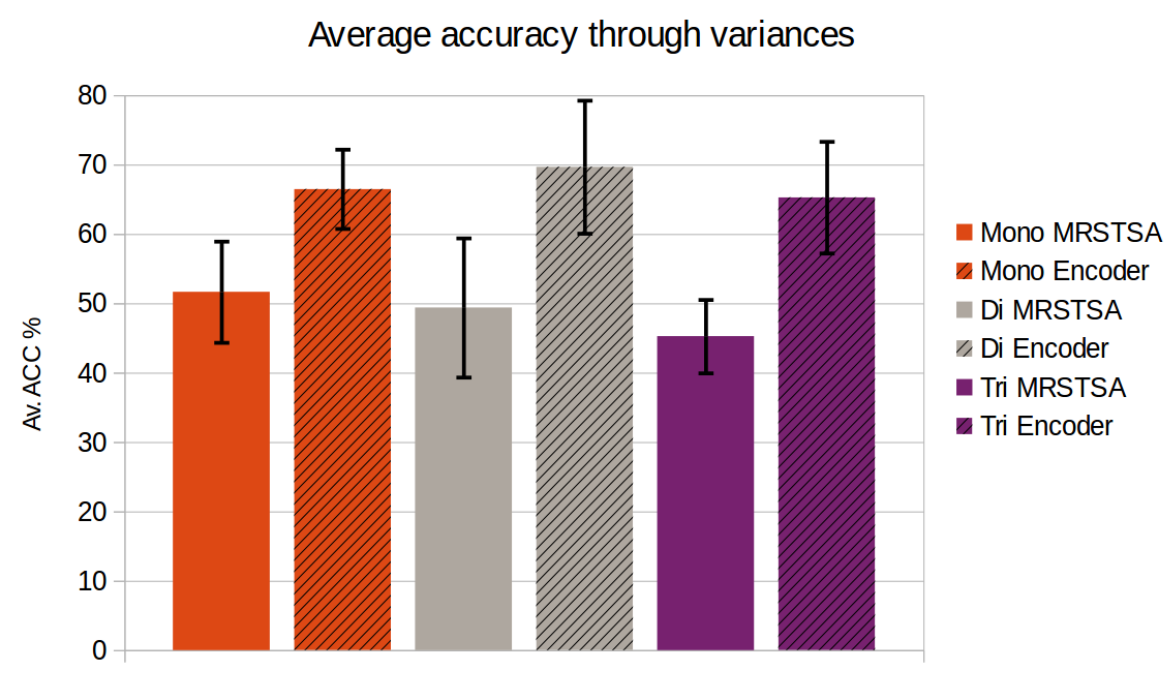
\includegraphics[width=1.0\textwidth]{WordClassification1.png}
    %\caption{Average classification accuracies across all acoustic variants for mono, di and trisyllabic words}
    %\label{fig:WordClassification1}
%\end{figure}


\end{appendices}

\end{document}
